\section{lexicographic-order \label{lexorder}}

%Cartesian Product or Lexicographic-Product



%In order to aid in later searches and intersections, an \textit{order} should be established.


%Along the sparse-index, the sparse-index-array is a series of tuples which represent the location of the data-entries.

%Sparse-tensor operations require searching and finding unique tuples in this index-array. Therefore we use a generalization of 1-dimensional sorting order which is the lexicographic-order. Here the tuples are put in a 1-dimensional order, and their corresponding elements are sorted (while permuting the entire tuple).


\subsection{array-of-tuples}

%The sparse-tensor's structure is given by their index-array. This may be seen as a collection of tuples.The tuples contain the numerical value of an index for each axis of a tensor, within the order of axës of the tensor. That is the tuples are ordered.

Numerical \textit{Lexicographic-order} is defined on a 2-dimensional array, a matrix (over some data-type), and we would like to sort along a given axis, say the columns, while preserving the rows. Alternatively, we may call this data-structure as a \textit{array-of-tuples}, in order to distinguish that the \textit{tuples'} order is preserved (rows), and we permute the \textit{array}, i.e. columns. We may denote this 2d array, array-of-tuples as: $A[ n | I ]$, for a \textit{array-index} (denoted by $I$) that acts \textit{row-wise} refers to the $I$th tuple, while acting \textit{column-wise} with a \textit{tuple-index} (denoted by $n$).


%In the computational environment, the collection of tuples forms a array (i.e. with an order) of tuples.

%we would like to distinguish array and tuples...

%Thus a generic sparse-tensor index-array is thus always a 2 dimensional array/matrix. 
%The canonical form of this array/matrix is set to have 
%The index-array's array-index corresponds 1-1 to a particular data entry.
%\caution




\subsection{tuple-tuple comparison \label{tuplecompare}}

Now we would like to define a notion of a tuple being smaller/larger than another, we denote this comparison by $\prec$ xor $\preceq$.
Suppose we have two tuples (of the same finite length, filled in with $n+1$ entries) $a, b \in \N^{n+1}$, then $a < b$ if we preform an element-wise subtraction $b - s = c$, and the first nonzero entry in $c$ (from left-to-right) is positive.
Equivalently, following \cite{Munkres}:
%\begin{align*}   (a[0], a[1], \cdots, a[n] ) &\prec (b[0], b[1], \cdots, b[n]) \\    \text{if } a[0] < b[0] \text{ , else } a[0] = b[0] \quad \text{\&}      \quad a[m] &< b[m] \,\,(\text{for } 0 < m \le n) \end{align*}
\begin{align*}
    (a[{0}], a[{1}], \cdots, a[{n}] ) &\prec (b[{0}], b[{1}], \cdots, b[{n}]) \\
    \text{starting left-to-right,   if } a[i] < b[i] \text{ , else } a_i = b_i \quad \text{\&}  
    \quad a[i+1] &< b[i+1] \,\,(\text{for } 0 < i \le n)\quad.
\end{align*}

\subsubsection{tuple-tuple equality}

Suppose we have two tuples (of the same size, filled in with $n+1$ entries) $a, b \in \N^{n+1}$, then $a = b$ iff $a[i] = b[i]$ for all $i$ (the $i$th element of $a$ matches the $i$th element of $b$).

\subsubsection{tuples-to-numbers}
Next we provide a comparison is useful for mapping tuples to a number-system, while maintaining order (given two tuples, if one is greater than the other, the corresponding numbers will also obey the relationship).
Suppose for a number-system we have radix/base $r$. Then we may map a tuple to number in this system (1-1) by the inner-product (superscripts here are the exponential operation, i.e. power):
\begin{align*}
\text{num}_r(a) &= a[n] * r^{n} + a[n-1] * r^{n-1} + \cdots + a[1] * r^1 + a[0] * r^0\quad\quad .
\end{align*}
E.g. the binary number-system $(r=2)$, decimal ($r=10$), duodecimal system $(r=12)$, hexadecimal $(r=16)$. It can be shown if $a<b$, then their numbers base $r$ also comply with $\text{num}_r(a) < \text{num}_r(b)$.





\subsection{definition of lexicographic/dictionary order}

%Last subsection we introduced the index-array, now we would like to arrange this array/matrix into a convenient form to facilitate searching. 

%Next, we would like to sort it's tuple entries, using the comparison of \S\ref{tuplecompare}, such that all tuples...\caution

%with the order of tuples remaining fixed. Therefore we would like to introduce a comparison of two tuples
%\subsubsection{lexicographic order}

A list-of-tuples (the index-array) is said to be \textit{lexicographically}-ordered if all pairs-of-tuples comply with the tuple-tuple comparison $\prec$. Note this does not include equality, and hence all entries must be unique, we denote this order as \textit{sssort} or \text{well-ordered} in a mathematical sense. 
%Index-arrays may also be indicated by 3-square brackets: $A\left[\!\left[\!\left[ \quad | \quad \right]\!\right]\!\right]$.
If we relax to equality in the comparison, we allow for duplicates and use the $\preceq$ comparison instead, this is denoted as \textit{ssort} order. %, or in symbolic notation as two-square-brackets $A\left[\!\left[ \quad | \quad \right]\!\right]$.


\begin{figure}[h!]
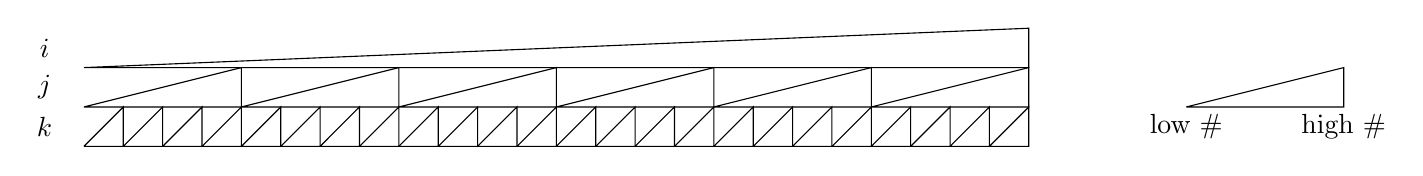
\begin{tikzpicture}
    \draw (0,0) -- (12,0) -- (12,0.5) -- (0,0);
    
    \draw ( 0,-0.5) -- ( 2,-0.5) -- ( 2, 0.0) -- ( 0,-0.5);
    \draw ( 2,-0.5) -- ( 4,-0.5) -- ( 4, 0.0) -- ( 2,-0.5);
    \draw ( 4,-0.5) -- ( 6,-0.5) -- ( 6, 0.0) -- ( 4,-0.5);
    \draw ( 6,-0.5) -- ( 8,-0.5) -- ( 8, 0.0) -- ( 6,-0.5);
    \draw ( 8,-0.5) -- (10,-0.5) -- (10, 0.0) -- ( 8,-0.5);
    \draw (10,-0.5) -- (12,-0.5) -- (12, 0.0) -- (10,-0.5);
    
    \draw (0.0,-1.0) -- (0.5,-1.0) -- (0.5,-0.5) -- ( 0.0,-1.0);
    \draw (0.5,-1.0) -- (1.0,-1.0) -- (1.0,-0.5) -- ( 0.5,-1.0);
    \draw (1.0,-1.0) -- (1.5,-1.0) -- (1.5,-0.5) -- ( 1.0,-1.0);
    \draw (1.5,-1.0) -- (2.0,-1.0) -- (2.0,-0.5) -- ( 1.5,-1.0);
    \draw (2.0,-1.0) -- (2.5,-1.0) -- (2.5,-0.5) -- ( 2.0,-1.0);
    \draw (2.5,-1.0) -- (3.0,-1.0) -- (3.0,-0.5) -- ( 2.5,-1.0);
    \draw (3.0,-1.0) -- (3.5,-1.0) -- (3.5,-0.5) -- ( 3.0,-1.0);
    \draw (3.5,-1.0) -- (4.0,-1.0) -- (4.0,-0.5) -- ( 3.5,-1.0);
    \draw (4.0,-1.0) -- (4.5,-1.0) -- (4.5,-0.5) -- ( 4.0,-1.0);
    \draw (4.5,-1.0) -- (5.0,-1.0) -- (5.0,-0.5) -- ( 4.5,-1.0);
    \draw (5.0,-1.0) -- (5.5,-1.0) -- (5.5,-0.5) -- ( 5.0,-1.0);
    \draw (5.5,-1.0) -- (6.0,-1.0) -- (6.0,-0.5) -- ( 5.5,-1.0);
    \draw (6.0,-1.0) -- (6.5,-1.0) -- (6.5,-0.5) -- ( 6.0,-1.0);
    \draw (6.5,-1.0) -- (7.0,-1.0) -- (7.0,-0.5) -- ( 6.5,-1.0);
    \draw (7.0,-1.0) -- (7.5,-1.0) -- (7.5,-0.5) -- ( 7.0,-1.0);
    \draw (7.5,-1.0) -- (8.0,-1.0) -- (8.0,-0.5) -- ( 7.5,-1.0);
    \draw (8.0,-1.0) -- (8.5,-1.0) -- (8.5,-0.5) -- ( 8.0,-1.0);
    \draw (8.5,-1.0) -- (9.0,-1.0) -- (9.0,-0.5) -- ( 8.5,-1.0);
    \draw (9.0,-1.0) -- (9.5,-1.0) -- (9.5,-0.5) -- ( 9.0,-1.0);
    \draw (9.5,-1.0) -- (10.0,-1.0) -- (10.0,-0.5) -- ( 9.5,-1.0);
    \draw (10.0,-1.0) -- (10.5,-1.0) -- (10.5,-0.5) -- ( 10.0,-1.0);
    \draw (10.5,-1.0) -- (11.0,-1.0) -- (11.0,-0.5) -- ( 10.5,-1.0);
    \draw (11.0,-1.0) -- (11.5,-1.0) -- (11.5,-0.5) -- ( 11.0,-1.0);
    \draw (11.5,-1.0) -- (12.0,-1.0) -- (12.0,-0.5) -- ( 11.5,-1.0);
    
    \draw ( 14,-0.5) -- ( 16,-0.5) -- ( 16, 0.0) -- ( 14,-0.5);
    \node(draw) at (14, -0.75)   (a) {low \#};
    \node(draw) at (16, -0.75)   (a) {high \#};
    \node(draw) at (-0.5, 0.25)   (a) {$i$};
    \node(draw) at (-0.5, -0.25)   (a) {$j$};
    \node(draw) at (-0.5, -0.75)   (a) {$k$};
    
\end{tikzpicture}
\caption{\label{ssortdiagram} 
A cartoon depicting the ordering of a list-of-tuples array for a 3-index $A[i,j,k | I]$, along $i$ numerical values are sorted in ascending-order. Afterward $j$ is sorted in ascending-order within duplicate-values in $i$ (the previous column). Lastly, $k$ is sorted in ascending-order within duplicate-values in $i$ and $j$ (both previous arrays.}
\end{figure}

%An array/list-of-tuples is said to be lexicographically \textit{ssorted}, given a tuple order and length 





%\caution we have an ordered set for indices, then apply this order ....

%\caution $i\in (S, \le)$

%Unique sets of tuples (of finite length without duplicates) are \textbf{well-ordered} in ssort. $ \prec,  \preceq,  \succ,  \succeq$

%Let tuples $a,b\in\N^\eta$, with $\eta$ ordered, then $b$ \textit{lexicographically-succeeds} $a$ (comes after), if the first nonzero number of: $a - b$ is negative.

%A set of tuples $A\in\N^\eta$ is said to be \textit{lexicographically-ssorted} with an enumeration given by $I$, if for-all elements in $A$, $A[I] \prec A[I']$ for $I < I'$.


%We have two comparisons $\ll$, $<$


%We like to view the index-array, of a sparse-tensor, as a list-of-tuples.






\subsubsection{lexicographic-sort algorithm}

Suppose we have a generic unsorted, potentially non-unique entry, list-of-tuples array (with column labels $\textbf{ 0, 1, 2, 3}, \cdots, \textbf{N}$):
\begin{align*}
    A\left[ \textbf{ 0, 1, 2, 3, }\cdots, \textbf{N} \,\,|\,I \,\right]\quad\quad.
\end{align*}
Next we introduce an auxiliary-array called the domain, $u$, which constrains the ranges of successive (column/index) sorts. For instance the sort is executed within successive elements in the domains array (range of list indices are [$u[n],u[n+1]$)), a constrained-sort:
\begin{align*}
    A\left[ \textbf{ 0, 1, 2, 3, }\cdots, \textbf{N} \,\,|\,\,u[n]\,:\,u[n+1]\,\,\right]\quad\quad.
\end{align*}

Upon sorting each index ($\textbf{0, 1, 2, 3}, \cdots, \textbf{N}$), the constrains on the sort are changed, and must increase. Initially there are no constraints. Then differences between the elements in the sorted index, form domains which constrains the sort of successive sorts.
Importantly, the domains $u^n$ must unionize with earlier domains $u^m$ ($m<n$) to respect earlier boundaries:
\begin{align*}
    u &= \bigcup_{\eta} \,u^{(\eta)}\quad\quad.
\end{align*} 
It would be convenient to have an \texttt{argsort} over small-domains, that can be parallelized over these small-domains.
This is quite natural for \texttt{mergesort} which partitions the data-set, before merging. Except we would like to specify this partition, which is potentially of different sizes. Then implement a sorting algorithm depending on the size of the partition: either \textit{Insertion-sort} xor \textit{Merge-sort}.


\subsubsection{computational time-complexity}

%Suppose after a sort we have $M$ domains of size $N/M$ (as total size needs to be $N$), we naively suspect this sorting algorithm to have computational-time-complexity: $\mathcal{O} \sim M  \left( \frac{N}{M}\log\frac{N}{M} \right) = N \log\left(\frac{N}{M}\right) $. As we go through the tuples- the number of domains increase...with $M^{(0)} = 1$ Let $M^{(\eta)} \sim M^\eta$
%\begin{align*} \mathcal{O} \sim    N \log N + N\log\left( \frac{N}{M^{(1)}} \right) + N\log\left( \frac{N}{M^{(2)}} \right) + \cdots + N\log\left( \frac{N}{M^{(\eta)}} \right) = N\left( \sum_{n\in\subset\N} \log\left( \frac{N}{M^{(\eta)}} \right) \right) \end{align*}



Let $N = M^n$ ($M$ is the length of a side of the dense-tensor), then we have to do successively constrained sort given by:
\begin{align*}
    \mathcal{O} &\sim
    M^n\left( \log{\left( \frac{M^n}{M^0} \right)} + \log{\left( \frac{M^n}{M^1} \right)} + \cdots + \log{\left( \frac{M^n}{M^n} \right)}\right) = \frac{n+1}{2} \,M^n\log{(M^n)} \\ &\sim \frac{n+1}{2} \,N\log{N}\quad\quad.
\end{align*}
Compare this to: $\mathcal{O}\sim n N\log N$, the independent sort of each column.





\subsubsection{theorems}

 %(assuming no permutation symmetries e.g. $123 \ne 132$).

The following may be easily shown:
\begin{itemize}
\item Adding an arbitrary (random) column to the right sssort-order order respects the original sssort-order.
\item Removing an arbitrary-row (a tuple) maintains sssort-order.
\item Removing an arbitrary-column in sssort-order breaks it to ssort-order (creating the possibility of duplicates).
\end{itemize}


